\section{Decision Trees (Programming)}

\subsection{Part 1: Effects of Dataset Size on Performance}
\begin{enumerate}
    \item Report the training, validation, and test accuracies on the full and partial datasets below. Note that this portion will be graded by the Autograder.
    \begin{center}
        \begin{tabular}{ |p{6cm}||p{3cm}|p{3cm}|  }
         \hline
         \multicolumn{3}{|c|}{Accuracy Scores} \\
         \hline
         & Full Dataset & Small Dataset\\
         \hline
         Training Accuracy   & 1.0    &1.0\\
         Validation Accuracy   & 0.7043478260869566    &0.7130434782608696\\
         Test Accuracy   & 0.7532467532467533    &0.6753246753246753\\
         \hline
        \end{tabular}
    \end{center}
    \item Which dataset had a higher difference between training and test accuracy? Briefly explain why.
    \newline
    \newline
    The small data set has a larger difference between test and validation accuracy. This is explained by over-fitting in the case of the partial data set. 
    $\ldots$
\end{enumerate}

\subsection{Part 2: Effects of Dataset Size on Performance}
\begin{enumerate}
    \item Report the chosen hyperparameters for the complete and partial set below. Note that this section will be graded by the Autograder.
    \begin{center}
        \begin{tabular}{ |p{6cm}||p{3cm}|p{3cm}|  }
         \hline
         \multicolumn{3}{|c|}{Grid Search Chosen Hyperparameters} \\
         \hline
         & Full Dataset & Small Dataset\\
         \hline
         Tree Depth   & 3    &1\\
         Max Leaf Nodes   & 4    &2\\
         \hline
        \end{tabular}
    \end{center}
    \item Did the small dataset have higher or lower chosen hyperparameter values than the full dataset? Briefly explain why.
    \newline
    \newline
    The small dataset has lower hyperparameters to combat its tendency to overfit.
    
\end{enumerate}

\subsection{Part 3: Retrain Decision Tree and Plot Hyperparameter Search}
\begin{enumerate}
    \item Report the train, validation, and test accuracies after retraining the decision tree with the new hyperparameters. Also paste in the values for the training and validation scores lists when varying the max leaf node count hyperparameter.
    \begin{center}
        \begin{tabular}{ |p{6cm}||p{3cm}|  }
         \hline
         \multicolumn{2}{|c|}{Retrained Decision Tree Performance for Small Dataset} \\
         \hline
         & Score\\
         \hline
         Training Accuracy   &0.8159722222222222\\
         Validation Accuracy     &0.7739130434782608\\
         Test Accuracy   &0.7142857142857143\\
         \hline
        \end{tabular}
    \end{center}
    \begin{center}
        \begin{tabular}{ |p{2cm}||p{7cm}|  }
         \hline
         \multicolumn{2}{|c|}{Training and Validation List Values} \\
         \hline
         & List\\
         \hline
         Training   &[0.7743, 0.7743, 0.7743, 0.7743, 0.7743, 0.7778, 0.7951, 0.8160, 0.8160]\\
         Validation &[0.7478, 0.7478, 0.7478, 0.7478, 0.7478, 0.7478, 0.7130, 0.7739, 0.7739]\\
         \hline
        \end{tabular}
    \end{center}
    \item  How did the training accuracy and testing accuracy change after tuning compared to before? Briefly explain why.
    \newline
    \newline
    The training accuracy decreased from $1.0 \to 0.82$ since the new model is no longer over-fitting. The testing accuracy increased from $0.66 \to 0.71$ for the same reason. Thus, with regularization hyper-parameters, the model fits the test data set better.
    
    \item Paste the plot of training and validation scores with different leaf count values on the small dataset. Explain any trends or patterns with the plot within validation and training scores and briefly explain why.
    
       \begin{figure}[H]
   	\centering
   	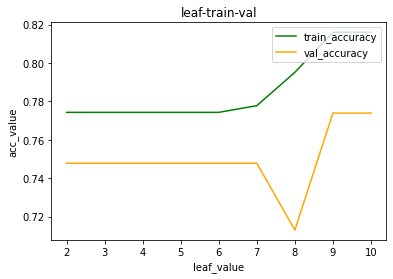
\includegraphics[width=0.4\textwidth]{images/decision_tree_programming.png}
   	\caption{Plot of training and validation scores.}
   	\label{fig:decision_tree_programming}
   \end{figure}
   
  The training accuracy is increasing and always higher than validation accuracy. The validation accuracy increases to a point since the increased leaf counts better capture the complexity of the model.
  
  Training accuracy will peak at a certain accuracy due to the max depth restriction.
    
\end{enumerate}
